\documentclass[
	letterpaper, % Paper size, specify a4paper (A4) or letterpaper (US letter)
	10pt, % Default font size, specify 10pt, 11pt or 12pt
]{CSUniSchoolLabReport}

%----------------------------------------------------------------------------------------
%	REPORT INFORMATION
%----------------------------------------------------------------------------------------

\title{Breadboards \\ Circuits \& Signals \\ EECE2150} % Report title

\author{Michael \textsc{Brodskiy}}

\date{January 17, 2023} % Date of the report

%----------------------------------------------------------------------------------------


\begin{document}

\maketitle % Insert the title, author and date using the information specified above

\begin{center}
	\begin{tabular}{l r}
		Date Performed: & January 9, 2023 \\ % Date the experiment was performed
        Partner: & Juan \textsc{Zapata} \\ % Partner names
		Instructor: & Professor \textsc{Sun} % Instructor/supervisor
	\end{tabular}
\end{center}

\section{Introduction}

The experiment that was undertaken concerned the analysis and physical reconstruction of basic electrical diagrams on a breadboard. The purpose of this was to familiarize ourselves with rudimentary functions of a breadboard.

\section{Experimental Data}

The voltage drops across each component were as follows:

\begin{center}
\begin{tabular}[h]{|c|c|}
  \hline
  Component & Voltage Drop [$\si{\volt}$]\\
  \hline
  Resistor 1 & 1.0708\\
  \hline
  Resistor 2 & 1.0708\\
  \hline
  LED 1 (Red) & 1.9511\\
  \hline
  LED 2 (Green) & 1.9811\\
  \hline
\end{tabular}
\end{center}

None of the measured voltages were negative for us; however, if we were to reverse the polarity (\textit{i.e.} switch the black and read voltmeter terminals), then the produced values would have the same magnitude but opposite sign.\\

The two LEDs did \underline{not} have the same voltage drop. The red LED had a drop of $1.9511[\si{\volt}]$ and the green one had a drop of $1.9811[\si{\volt}]$\\

The circuits constructed did all work on the first try; however, real-world circuits, which are significantly more complex, almost definitely do not work on the first try.

\section{Constructed Circuits}

\begin{multicols}{2}

\begin{figure}[H]
  \centering
  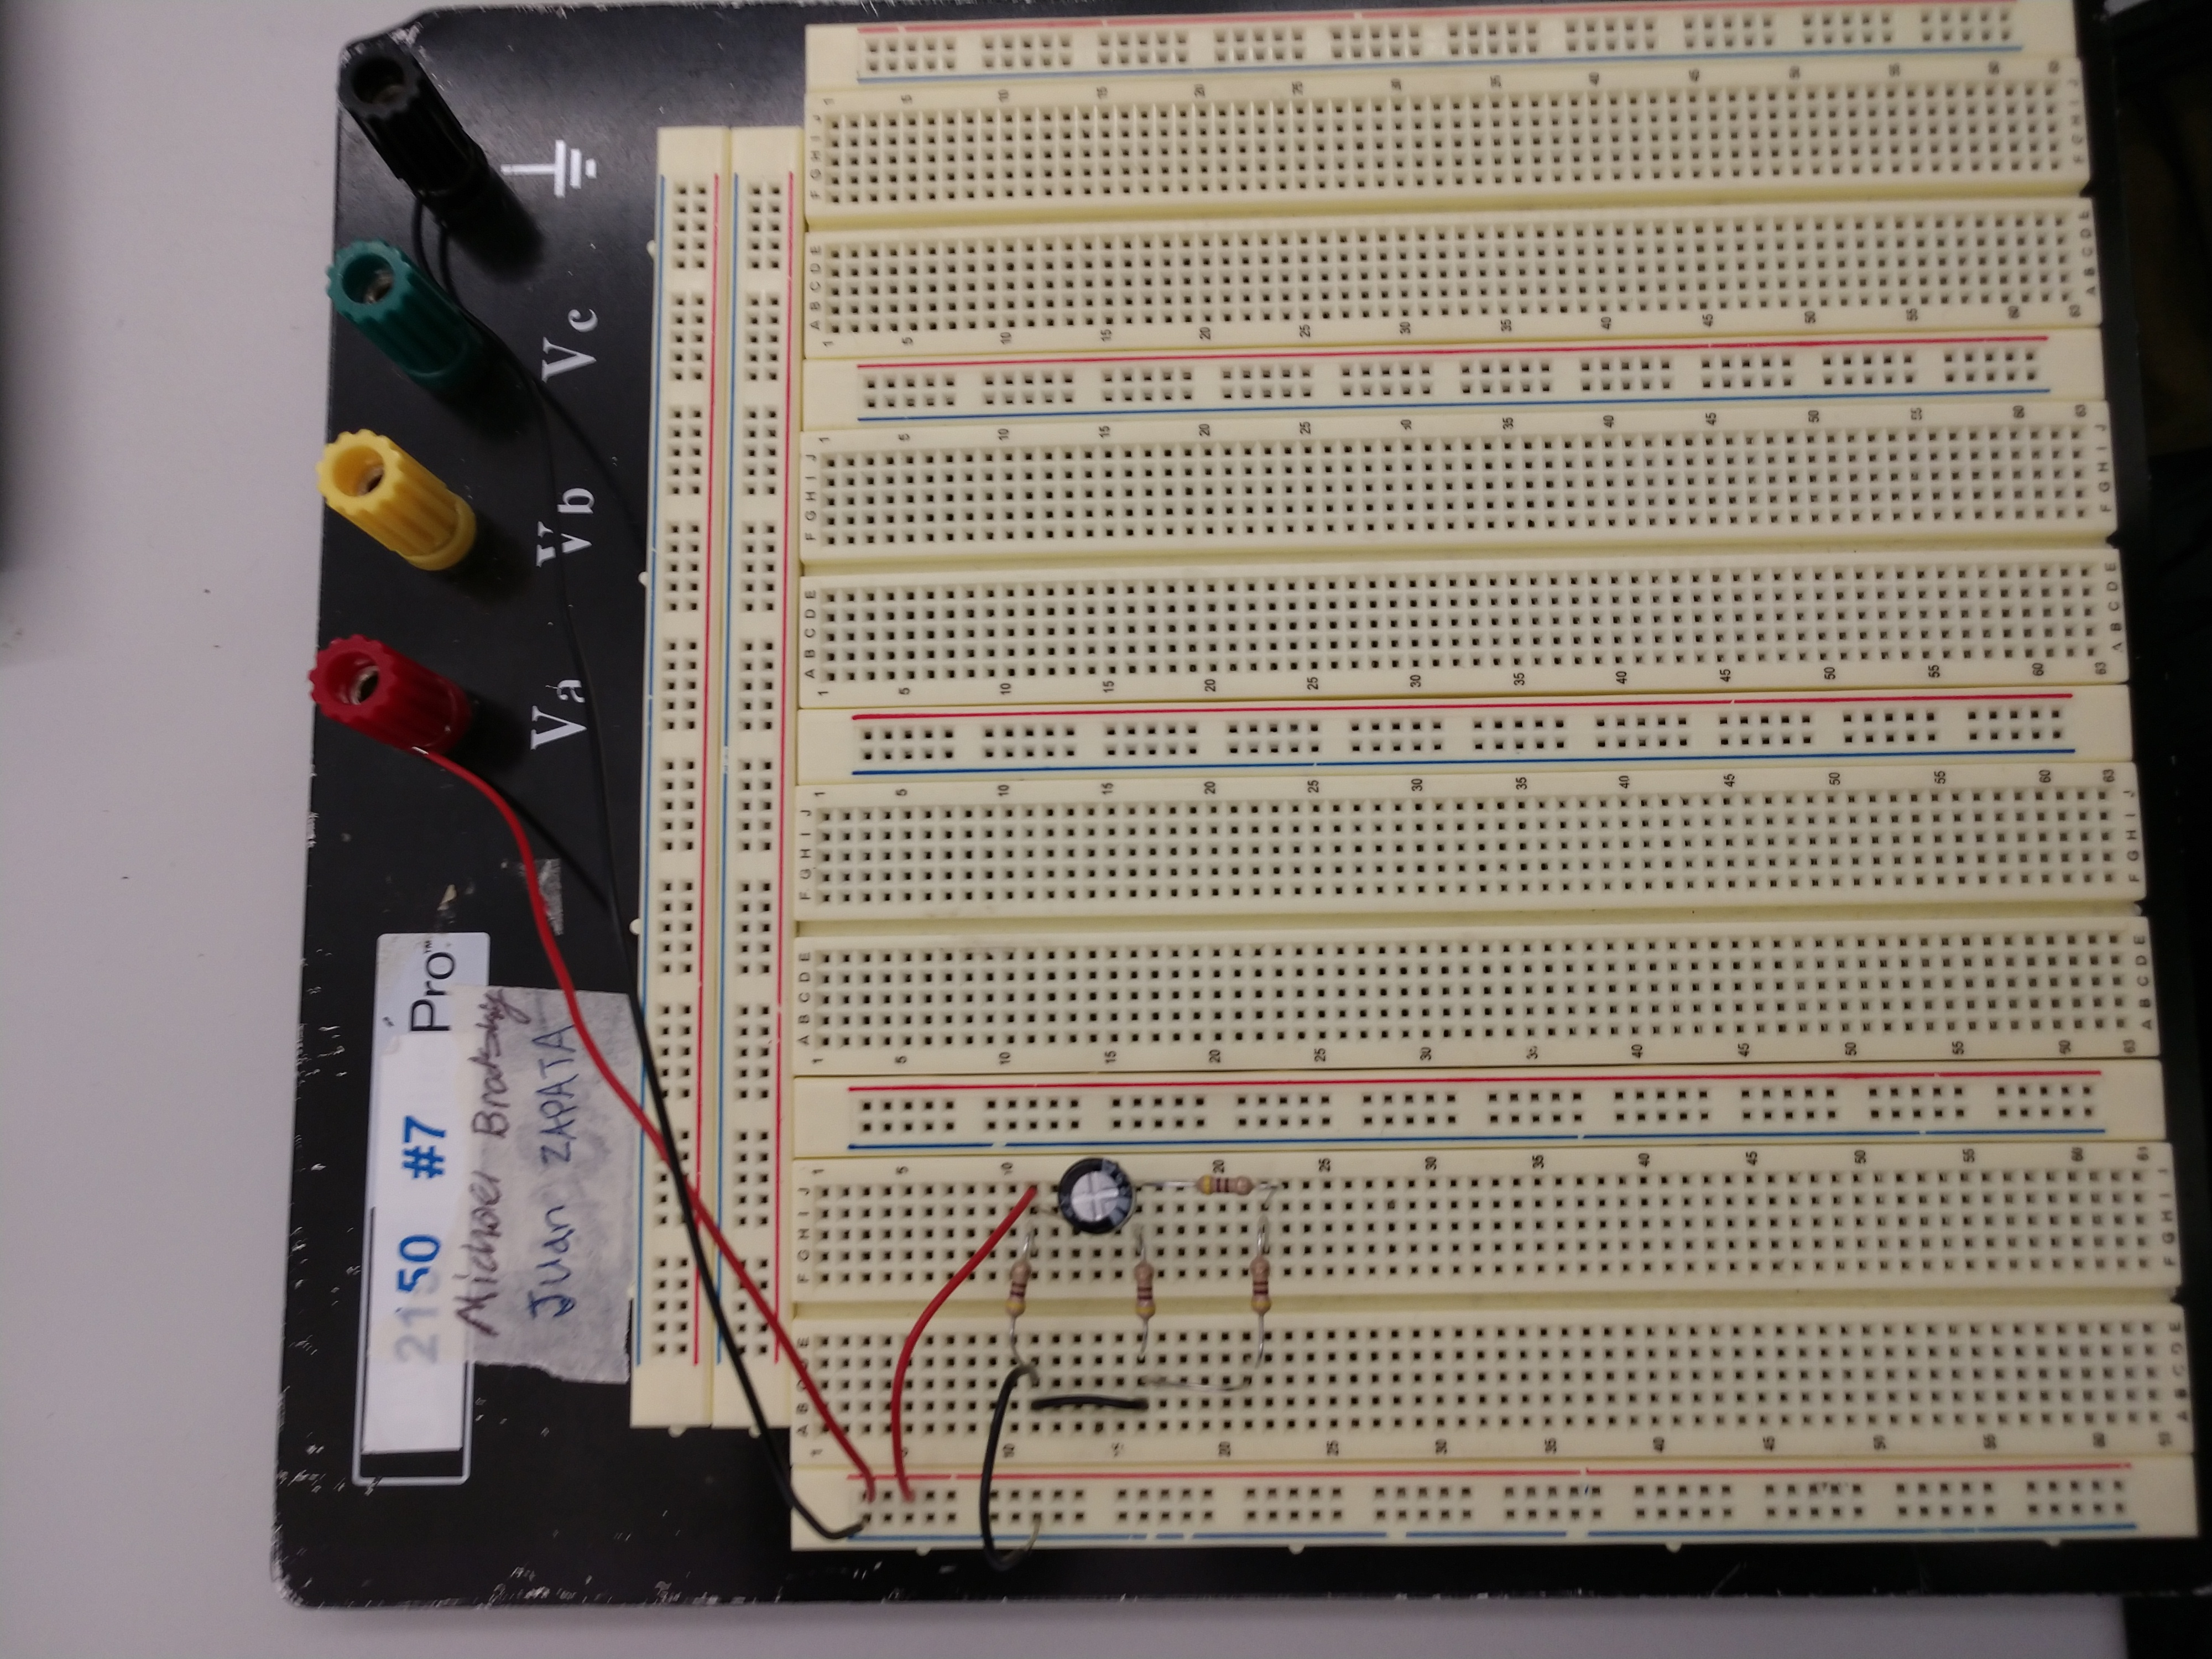
\includegraphics[width=.45\textwidth]{Figures/L1C1.jpg}\\
  \caption{Circuit 1 Implementation}
  \label{fig:1}
\end{figure}\\

\begin{figure}[H]
  \centering
  \tikzset{every picture/.style={line width=0.75pt}} %set default line width to 0.75pt        

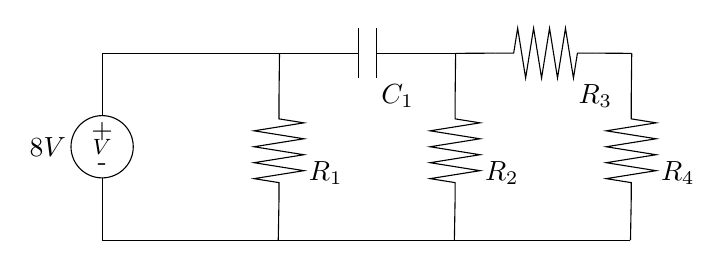
\begin{tikzpicture}[x=0.75pt,y=0.75pt,yscale=-.6,xscale=.6]
%uncomment if require: \path (0,536); %set diagram left start at 0, and has height of 536

%Shape: Resistor [id:dp4889124512217269] 
\draw   (267,193.2) -- (267,178.8) -- (247,175.6) -- (287,169.2) -- (247,162.8) -- (287,156.4) -- (247,150) -- (287,143.6) -- (247,137.2) -- (287,130.8) -- (267,127.6) -- (267,113.2) ;
%Shape: Resistor [id:dp8283103129084957] 
\draw   (549.84,113.2) -- (549.84,127.6) -- (569.84,130.8) -- (529.84,137.2) -- (569.84,143.6) -- (529.84,150) -- (569.84,156.4) -- (529.84,162.8) -- (569.84,169.2) -- (529.84,175.6) -- (549.84,178.8) -- (549.84,193.2) ;
%Shape: Resistor [id:dp7571735122141612] 
\draw   (441.06,74.82) -- (455.46,74.82) -- (458.66,54.82) -- (465.06,94.82) -- (471.46,54.82) -- (477.86,94.82) -- (484.26,54.82) -- (490.66,94.82) -- (497.06,54.82) -- (503.46,94.82) -- (506.66,74.82) -- (521.06,74.82) ;
%Shape: Circle [id:dp2948942053580248] 
\draw   (100,150) .. controls (100,136.19) and (111.19,125) .. (125,125) .. controls (138.81,125) and (150,136.19) .. (150,150) .. controls (150,163.81) and (138.81,175) .. (125,175) .. controls (111.19,175) and (100,163.81) .. (100,150) -- cycle ;
%Straight Lines [id:da9703905405516369] 
\draw    (125,175) -- (125,225) ;
%Straight Lines [id:da43407919574552967] 
\draw    (125,75) -- (125,125) ;
%Straight Lines [id:da17971604462169766] 
\draw    (267.42,75) -- (125,75) ;
%Straight Lines [id:da5657229854791843] 
\draw    (266.42,225) -- (125,225) ;
%Straight Lines [id:da4896240062556665] 
\draw    (267.42,75) -- (267,113.2) ;
%Straight Lines [id:da7708532745708458] 
\draw    (267,193.2) -- (266.42,225) ;
%Shape: Resistor [id:dp25386195284303326] 
\draw   (408.42,193.2) -- (408.42,178.8) -- (388.42,175.6) -- (428.42,169.2) -- (388.42,162.8) -- (428.42,156.4) -- (388.42,150) -- (428.42,143.6) -- (388.42,137.2) -- (428.42,130.8) -- (408.42,127.6) -- (408.42,113.2) ;
%Straight Lines [id:da660859645592087] 
\draw    (408.84,75) -- (408.42,113.2) ;
%Straight Lines [id:da8245190655595378] 
\draw    (408.42,193.2) -- (407.84,225) ;
%Straight Lines [id:da5852450560290101] 
\draw    (407.84,225) -- (266.42,225) ;
%Straight Lines [id:da46536937531365385] 
\draw    (549.26,225) -- (407.84,225) ;
%Straight Lines [id:da9277628078248175] 
\draw    (549.84,193.2) -- (549.26,225) ;
%Straight Lines [id:da13081367907412988] 
\draw    (550.26,75) -- (549.84,113.2) ;
%Straight Lines [id:da5576014517772203] 
\draw    (550.26,75) -- (521.06,74.82) ;
%Straight Lines [id:da6384607709236478] 
\draw    (441.06,74.82) -- (408.84,75) ;
%Shape: Capacitor [id:dp639148669096967] 
\draw   (267.42,75) -- (331.06,75) (345.2,55) -- (345.2,95) (331.06,55) -- (331.06,95) (345.2,75) -- (408.84,75) ;

% Text Node
\draw (98,150) node [anchor=east] [inner sep=0.75pt]   [align=left] {8$\displaystyle V$};
% Text Node
\draw (125,128) node [anchor=north] [inner sep=0.75pt]   [align=left] {\begin{minipage}[lt]{8.68pt}\setlength\topsep{0pt}
\begin{center}
+
\end{center}

\end{minipage}};
% Text Node
\draw (125,150) node  [font=\footnotesize] [align=left] {$\displaystyle V$};
% Text Node
\draw (125,172) node [anchor=south] [inner sep=0.75pt]   [align=left] {\begin{minipage}[lt]{8.67pt}\setlength\topsep{0pt}
\begin{center}
\mbox{-}
\end{center}

\end{minipage}};
% Text Node
\draw (289,159.4) node [anchor=north west][inner sep=0.75pt]   [align=left] {$\displaystyle R_{1}$};
% Text Node
\draw (430.42,159.4) node [anchor=north west][inner sep=0.75pt]   [align=left] {$\displaystyle R_{2}$};
% Text Node
\draw (505.46,97.82) node [anchor=north west][inner sep=0.75pt]   [align=left] {$\displaystyle R_{3}$};
% Text Node
\draw (571.84,159.4) node [anchor=north west][inner sep=0.75pt]   [align=left] {$\displaystyle R_{4}$};
% Text Node
\draw (347.2,98) node [anchor=north west][inner sep=0.75pt]   [align=left] {$\displaystyle C_{1}$};


\end{tikzpicture}

  \caption{Circuit 1 Diagram}
  \label{fig:2}
\end{figure}

\end{multicols}

\begin{multicols}{2}

\begin{figure}[H]
  \centering
  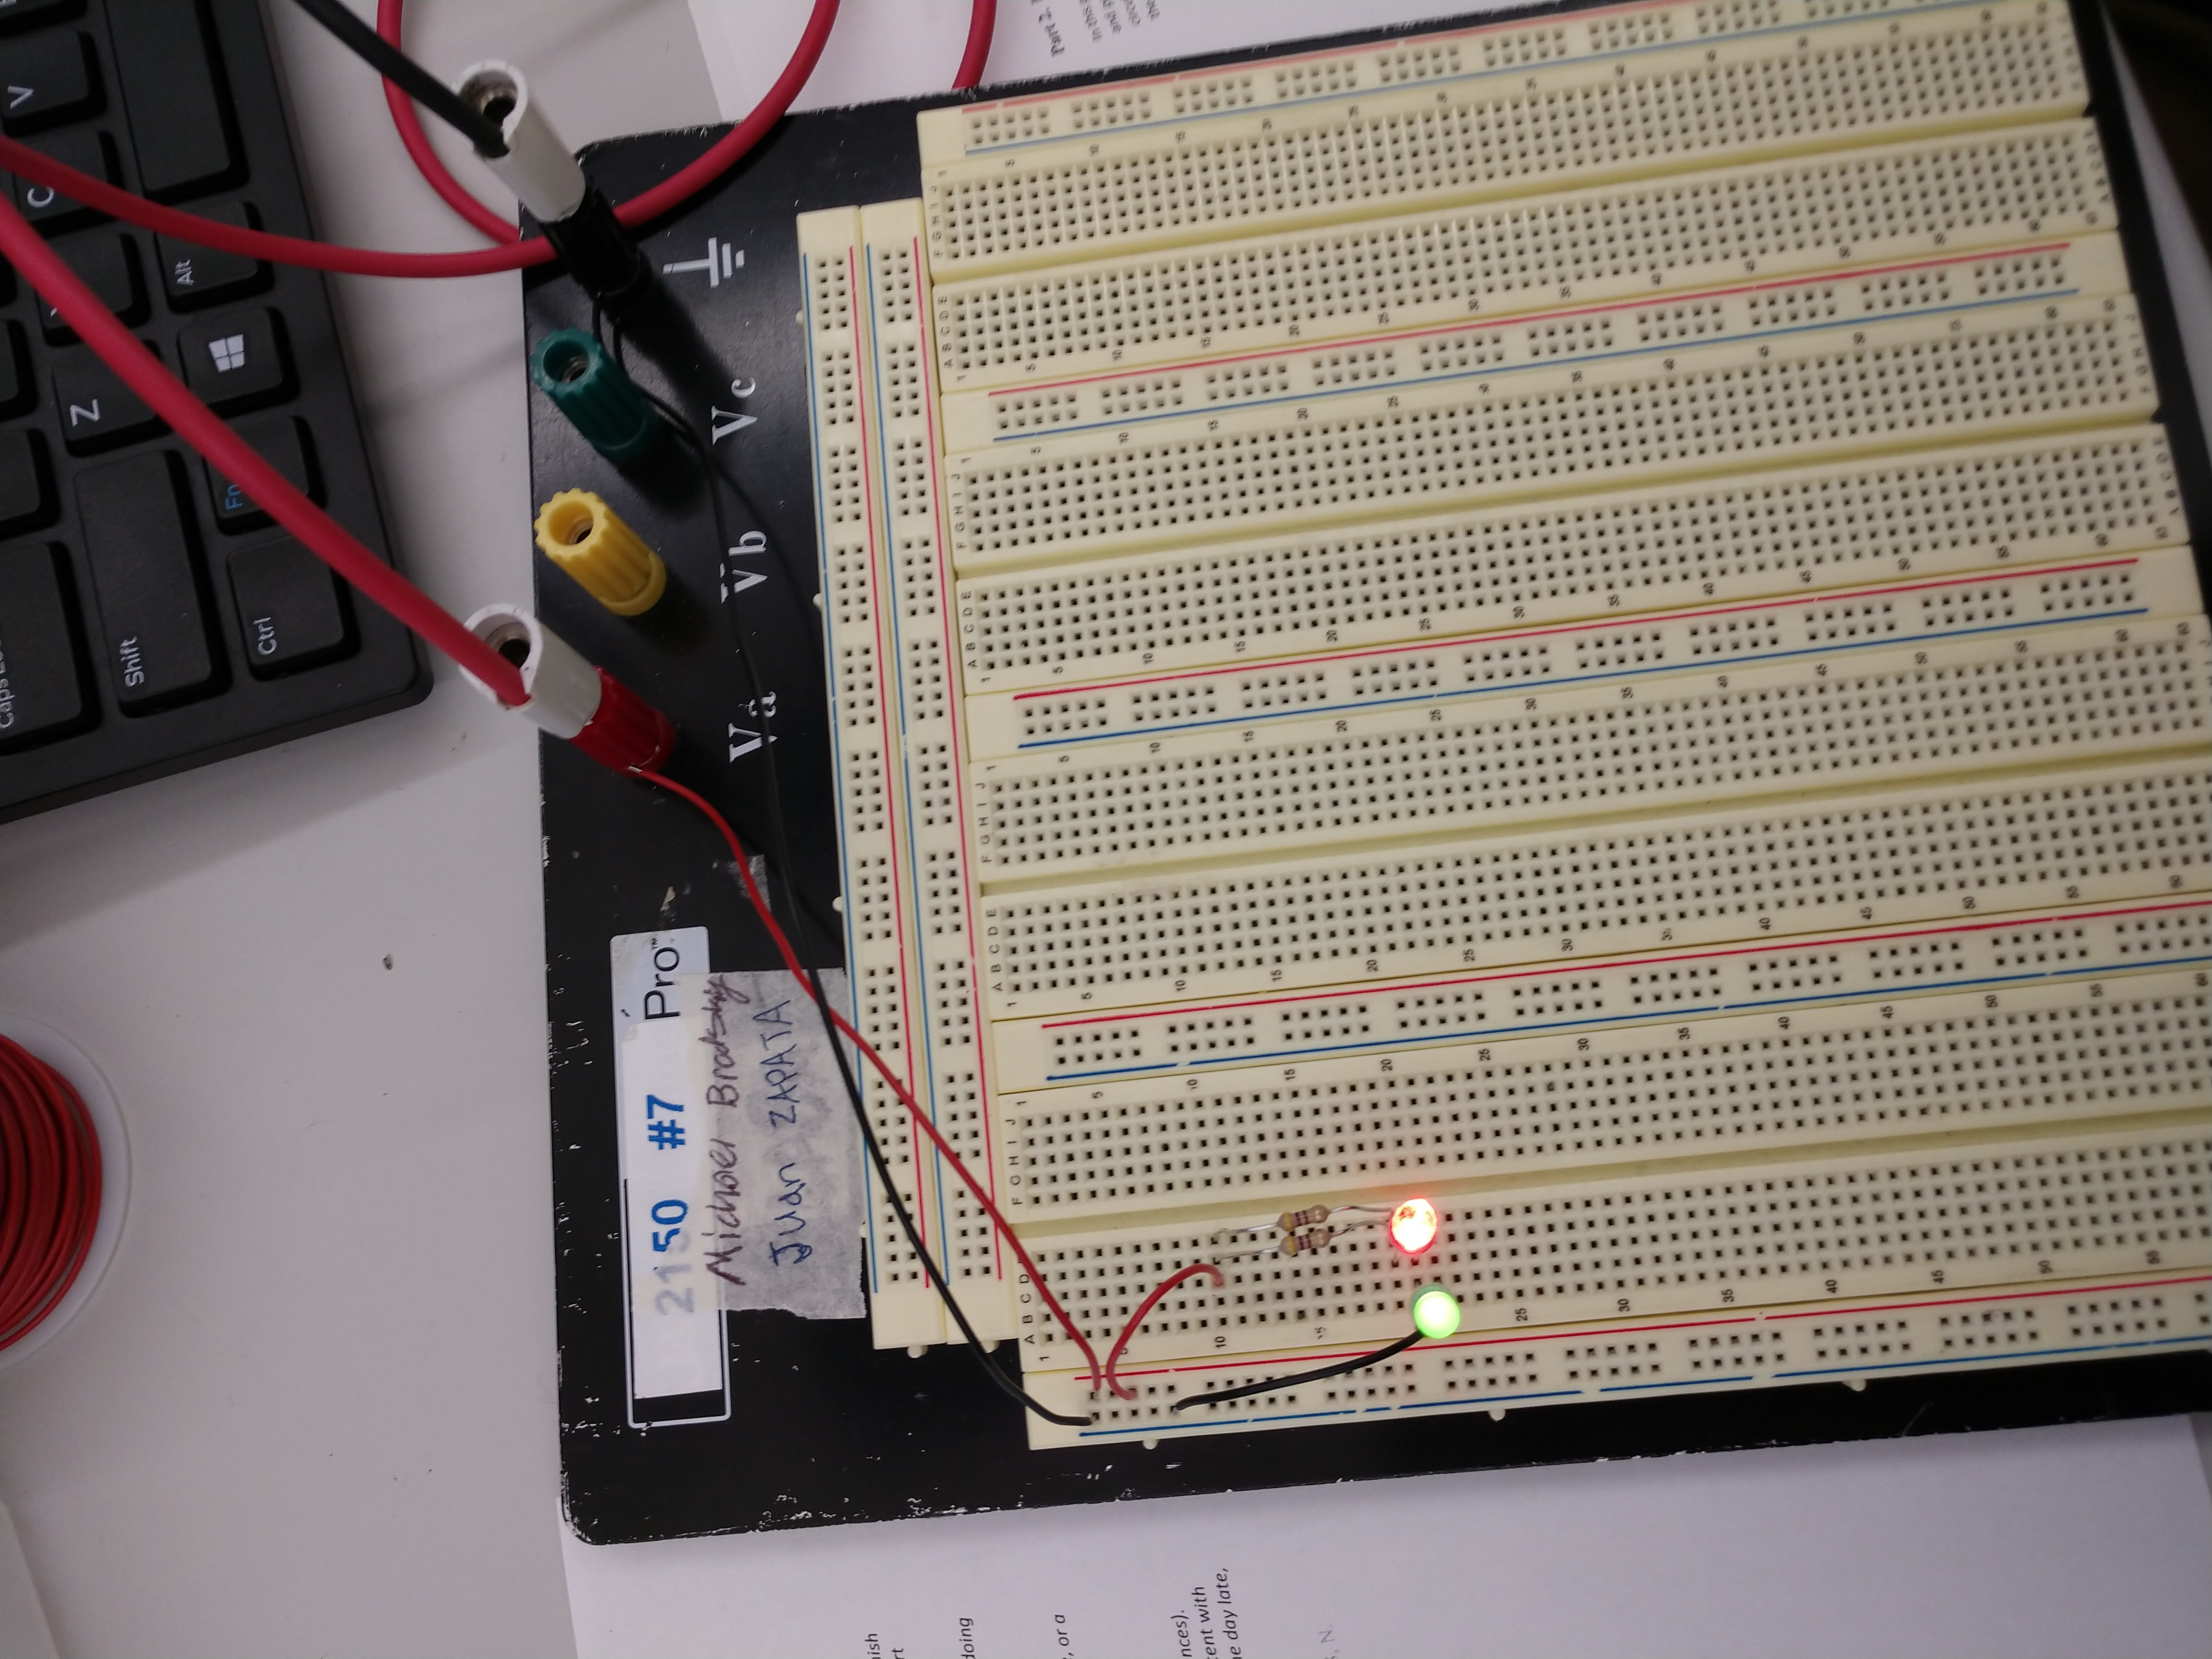
\includegraphics[width=.45\textwidth]{Figures/L1C2.jpg}
  \caption{Circuit 2 Implementation}
  \label{fig:3}
\end{figure}

\begin{figure}[H]
  \centering
  \tikzset{every picture/.style={line width=0.75pt}} %set default line width to 0.75pt        

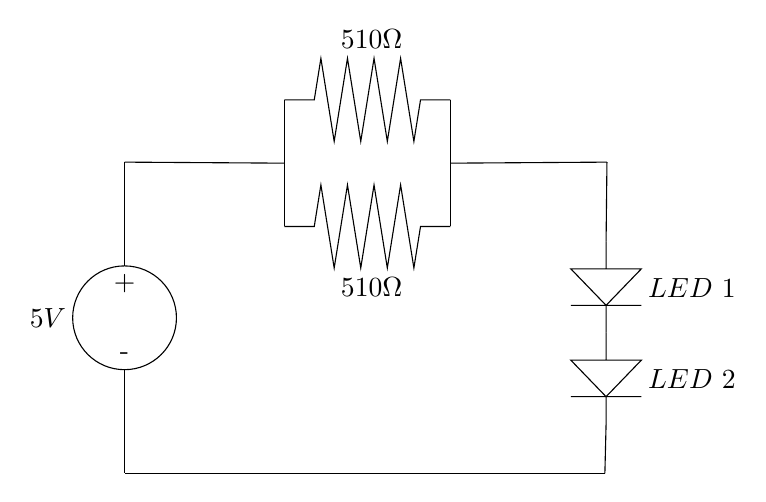
\begin{tikzpicture}[x=0.75pt,y=0.75pt,yscale=-1,xscale=1]
%uncomment if require: \path (0,536); %set diagram left start at 0, and has height of 536

%Shape: Circle [id:dp5391891321479709] 
\draw   (100,150) .. controls (100,136.19) and (111.19,125) .. (125,125) .. controls (138.81,125) and (150,136.19) .. (150,150) .. controls (150,163.81) and (138.81,175) .. (125,175) .. controls (111.19,175) and (100,163.81) .. (100,150) -- cycle ;
%Straight Lines [id:da29466546451147524] 
\draw    (125,175) -- (125,225) ;
%Straight Lines [id:da8075537755444633] 
\draw    (125,75) -- (125,125) ;
%Straight Lines [id:da5849282817970671] 
\draw    (357.42,75) -- (357,113.2) ;
%Straight Lines [id:da12428704129603618] 
\draw    (357,201.2) -- (356.42,225) ;
%Shape: Resistor [id:dp8585859917231262] 
\draw   (202,45) -- (216.4,45) -- (219.6,25) -- (226,65) -- (232.4,25) -- (238.8,65) -- (245.2,25) -- (251.6,65) -- (258,25) -- (264.4,65) -- (267.6,45) -- (282,45) ;
%Shape: Resistor [id:dp15449677573718512] 
\draw   (202,106) -- (216.4,106) -- (219.6,86) -- (226,126) -- (232.4,86) -- (238.8,126) -- (245.2,86) -- (251.6,126) -- (258,86) -- (264.4,126) -- (267.6,106) -- (282,106) ;
%Straight Lines [id:da07488249960137638] 
\draw    (202,45) -- (202,106) ;
%Straight Lines [id:da5526259810987513] 
\draw    (282,45) -- (282,106) ;
%Straight Lines [id:da2112986632937388] 
\draw    (125,75) -- (202,75.5) ;
%Straight Lines [id:da0027222316083801434] 
\draw    (282,75.5) -- (357.42,75) ;
%Shape: Diode [id:dp28676301231572787] 
\draw   (374,126.4) -- (357,144) -- (340,126.4) -- (374,126.4) -- cycle (357,113.2) -- (357,126.4) (374,144) -- (340,144) (357,144) -- (357,157.2) ;
%Shape: Diode [id:dp4391606122805669] 
\draw   (374,170.4) -- (357,188) -- (340,170.4) -- (374,170.4) -- cycle (357,157.2) -- (357,170.4) (374,188) -- (340,188) (357,188) -- (357,201.2) ;

%Straight Lines [id:da5657229854791843] 
\draw    (356.42,225) -- (125,225) ;

% Text Node
\draw (98,150) node [anchor=east] [inner sep=0.75pt]   [align=left] {5$\displaystyle V$};
% Text Node
\draw (125,128) node [anchor=north] [inner sep=0.75pt]   [align=left] {\begin{minipage}[lt]{8.68pt}\setlength\topsep{0pt}
\begin{center}
+
\end{center}

\end{minipage}};
% Text Node
\draw (125,172) node [anchor=south] [inner sep=0.75pt]   [align=left] {\begin{minipage}[lt]{8.67pt}\setlength\topsep{0pt}
\begin{center}
\mbox{-}
\end{center}

\end{minipage}};
% Text Node
\draw (228,129.4) node [anchor=north west][inner sep=0.75pt]    {$510\Omega $};
% Text Node
\draw (228,21.6) node [anchor=south west] [inner sep=0.75pt]    {$510\Omega $};
% Text Node
\draw (376,129.8) node [anchor=north west][inner sep=0.75pt]    {$LED\ 1$};
% Text Node
\draw (376,173.8) node [anchor=north west][inner sep=0.75pt]    {$LED\ 2$};


\end{tikzpicture}

  \caption{Circuit 2 Diagram}
  \label{fig:4}
\end{figure}

\end{multicols}

\section{Conclusion}

Overall, breadboards seem to be a good substitute for soldering, especially when constructing the simple circuits shown above. Additionally, it is logical that the green LED would consume more volts, as green is higher on the photon energy spectrum than red, and, as such, would take more volts to power.

\end{document}
